% Analyse
\section{Analyse}\label{sec:analyse}
Es gibt auch die Möglichkeit, zwei Bilder direkt nebeneinander darzustellen:

  \begin{figure} [ht]
    \centering
    \begin{subfigure}[b]{0.45\textwidth}
        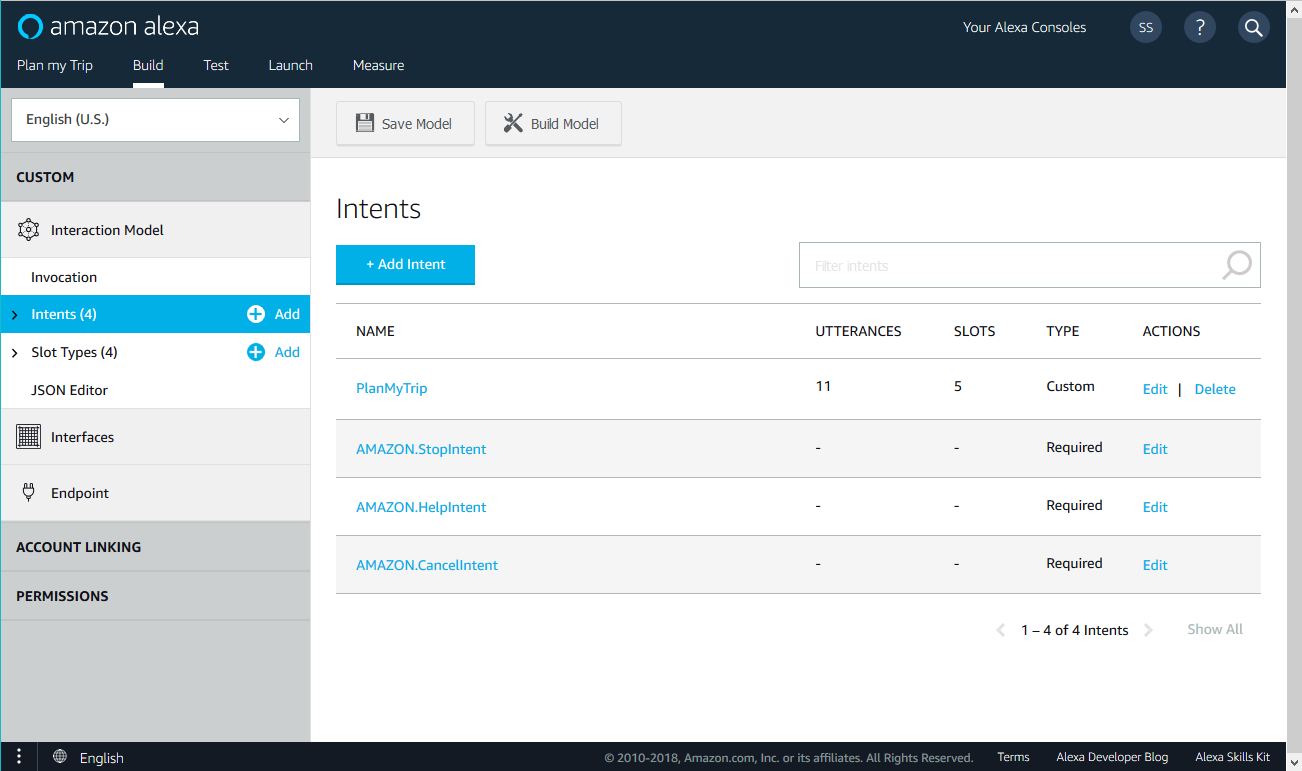
\includegraphics[width=\textwidth]{resources/images/amazon_dev_console.png}
        \caption{Beispielbild4}
        \label{fig:bild4}
    \end{subfigure}
    ~
    \begin{subfigure}[b]{0.45\textwidth}
        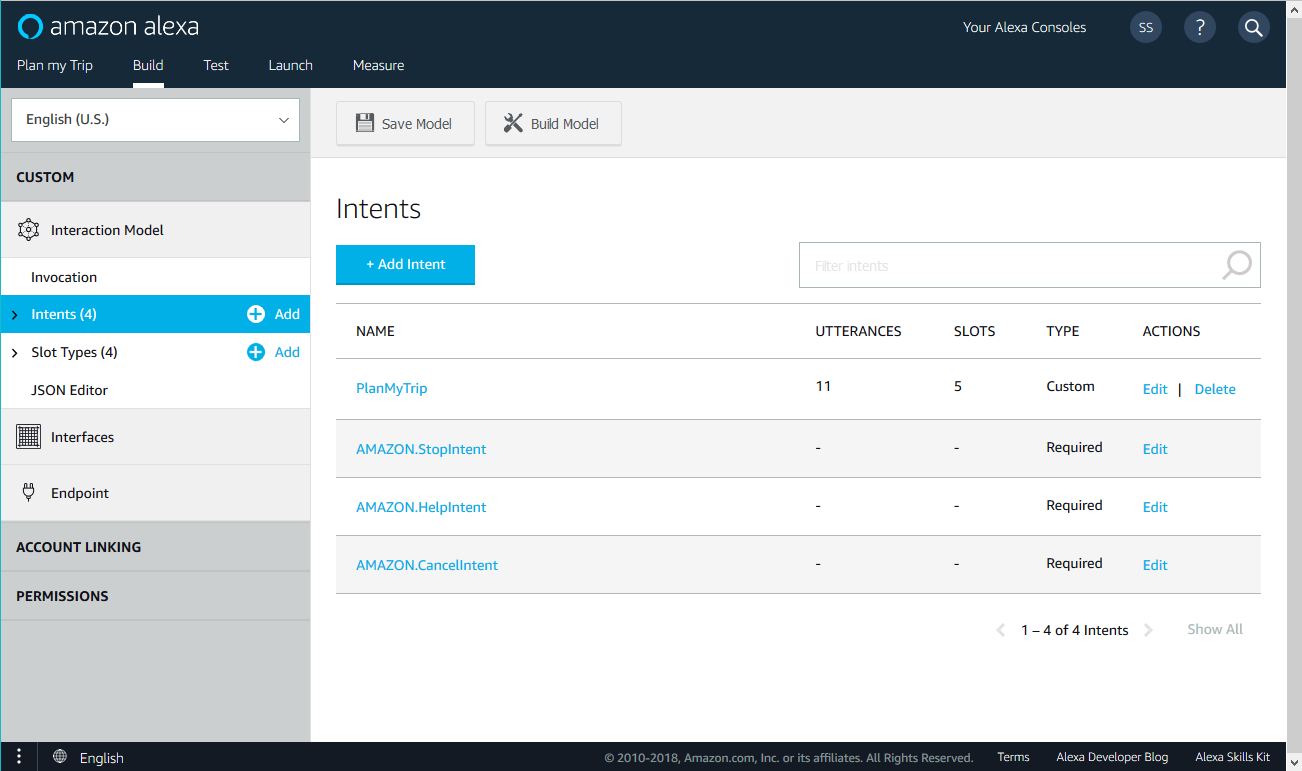
\includegraphics[width=\textwidth]{resources/images/amazon_dev_console.png}
        \caption{Beispielbild4}
        \label{fig:bild5}
    \end{subfigure}
    \caption{Zusammenstellung mehrerer Bilder}\label{fig:bild6}
\end{figure}